\chapter{强化学习的心理学} \label{chap:chap11}

在前面的章节中,我们仅基于计算考虑就提出了算法的想法。
在本章中,我们从另一个角度来看其中的一些算法:心理学的角度及其对动物如何学习的研究。
本章的目的是,首先,讨论强化学习的思想和算法与心理学家对动物学习的发现相对应的方式,其次,解释强化学习对动物学习研究的影响。
事实证明,强化学习提供的清晰形式主义将任务,回报和算法系统化,在理解实验数据,提出新的实验种类以及指出可能对操作和测量至关重要的因素方面非常有用。
长期优化回报的想法是强化学习的核心,这有助于我们理解动物学习和行为的其他令人困惑的特征。


强化学习与心理学理论之间的一些对应关系并不令人惊讶,因为强化学习的发展受到了心理学学习理论的启发。
然而,正如本书所述,强化学习从人工智能研究人员或工程师的角度探索理想化的情况,目的是用有效的算法解决计算问题,而不是复制或详细解释动物如何学习。
因此,我们描述的一些通信将各自领域中独立产生的想法联系起来。
我们认为这些接触点特别有意义,因为它们揭示了对学习很重要的计算原理,无论是通过人工还是通过自然系统学习。


在大多数情况下,我们描述了强化学习和学习理论之间的对应关系,这些理论是为了解释大鼠,鸽子和兔子等动物如何在受控实验室实验中学习而开发的。
在整个20世纪进行了数千次这样的实验,其中许多至今仍在进行中。
虽然有时被认为与心理学中更广泛的问题无关,但这些实验探索了动物学习的微妙特性,通常是由精确的理论问题驱动的。
随着心理学将重点转移到行为的更多认知方面,即思维和推理等心理过程,动物学习实验在心理学中的作用比以前少了。
但是,这项实验导致了学习原则的发现,这些原则在整个动物界都是基本的和广泛的,这些原则在设计人工学习系统时不应该被忽视。
此外,正如我们将看到的那样,认知处理的某些方面自然地与强化学习提供的计算视角相关联。


本章的最后一节包括与我们讨论的联系以及我们忽视的联系相关的参考文献。
我们希望本章鼓励读者更深入地探讨所有这些联系。
最后一节还讨论了强化学习中使用的术语与心理学术语的关系。
强化学习中使用的许多术语和短语都是从动物学习理论中借用的,但是这些术语和短语的计算/工程意义并不总是与其在心理学中的意义一致。


\section{预测和控制}


我们在本书中描述的算法分为两大类:预测算法和控制算法。
这些类别自然出现在强化学习问题的解决方法中。
在许多方面,这些类别分别对应于心理学家广泛研究的学习类别:经典或巴甫洛夫式条件作用和工具性或操作性条件作用。
由于心理学对强化学习的影响,这些对应关系并不完全是偶然的,但它们仍然引人注目,因为它们将来自不同目标的想法联系起来。


本书中介绍的预测算法估计的数量取决于代理环境的特征在未来的发展情况。
我们特别关注于估计代理在与环境交互时未来可能获得的回报量。
在这个角色中,预测算法是策略评估算法,它是改进策略算法的组成部分。
但预测算法不仅限于预测未来的回报;他们可以预测环境的任何特征(例如,参见Modayil,White和Sutton,2014)。
预测算法和经典条件反射之间的对应关系取决于它们预测即将到来的刺激的共同特性,无论这些刺激是否有益(或惩罚)。


仪器或操作条件实验的情况是不同的。
在这里,实验装置的设置是为了根据动物的行为给予动物喜欢的东西(奖励)或不喜欢的东西(惩罚)。
动物学会增加产生奖励行为的倾向,减少产生惩罚行为的倾向。
据说强化刺激取决于动物的行为,而在经典条件反射中则不然(尽管在经典条件反射实验中很难消除所有行为偶然性)。
仪器调节实验就像我们在第一章中简要讨论的那些启发桑代克效应定律的实验。
控制是这种学习形式的核心,它对应于强化学习的策略改进算法的操作。


在预测方面思考经典条件反射,在控制方面思考工具条件反射,是将我们的强化学习的计算观点与动物学习联系起来的起点,但实际上,情况比这更复杂。
经典条件作用比预测更多;它还涉及行动,控制模式也是如此,有时被称为巴甫洛夫控制。
此外,经典和工具性条件反射以有趣的方式相互作用,这两种学习都可能在大多数实验情况下进行。
尽管存在这些复杂性,但将经典/工具区别与预测/控制区别相结合是将强化学习与动物学习联系起来的方便的rst近似。


在心理学中,强化一词用于描述经典条件反射和工具条件反射的学习。
最初只指强化一种行为模式,也经常用于弱化一种行为模式。
被认为是行为改变原因的刺激被称为增强剂,它是否取决于动物以前的行为。
在本章的末尾,我们将更详细地讨论这个术语,以及它与机器学习中使用的术语的关系。


\section{经典条件反射}

在研究消化系统的活动时,著名的俄罗斯生理学家伊万·巴甫洛夫(IvanPavlov)发现,动物对某些触发刺激的先天反应可能会被与先天触发因素无关的其他刺激触发。
他的实验对象是经过小手术的狗,以准确测量其唾液re-ex的强度。
在他描述的一个案例中,这只狗在大多数情况下都不会流涎,但在喂食后约5秒钟,它会在接下来的几秒钟内产生约6滴唾液。
在几次重复呈现另一种刺激后,一种与食物无关的刺激,在这种情况下是节拍器的声音,在引入食物之前不久,狗对节拍器的声音做出了唾液分泌的反应,就像它对食物的反应一样。
“因此,唾液腺的活动被声音的冲动所激发,这是一种与食物完全不同的刺激”(巴甫洛夫,1927,第22页)。
巴甫洛夫总结了这一发现的重要性,写道:


很明显,在自然条件下,正常动物不仅必须对自身带来直接好处或伤害的刺激作出反应,而且还必须对其他物理或化学机构(声波,光波等)作出反应,这些物理或化学机构本身只发出这些刺激的接近信号;
虽然猎物的视觉和声音本身对较小的动物有害,但它的牙齿和爪子有害。(巴甫洛夫,1927年,第14页)


以这种方式将新刺激与先天性反应联系起来,现在被称为经典或巴甫洛夫条件反射。
巴甫洛夫(或者更确切地说,他的翻译人员)将先天性反应(例如,上述演示中的流涎)称为“无条件反应”(URs),其自然触发刺激(例如食物)“无条件刺激”(USs),以及由预测刺激触发的新反应(例如,这里还有流涎)“条件反应”(CRs)。
最初是中性的刺激,意味着它通常不会引起强烈的反应(例如节拍器声音),当动物知道它预测美国并因此产生CR以响应CS时,它就会成为“条件刺激”(CS)。
这些术语仍然用于描述经典的条件反射实验(尽管更好的翻译应该是“有条件的”和“无条件的”,而不是有条件的和无条件的)。
美国被称为强化者,因为它强化了对CS产生CR的反应。


右侧显示了两种常见类型的经典调节实验中刺激的排列。
在延迟调节中,CS延伸到整个刺激间隔或ISI,这是CS发作和美国发作之间的时间间隔(当美国以此处显示的常见版本结束时,CS结束)。
在跟踪条件反射中,US在CS结束后开始,CS o集合和US开始之间的时间间隔称为跟踪间隔。


\begin{figure}[!htb]
	\centering
	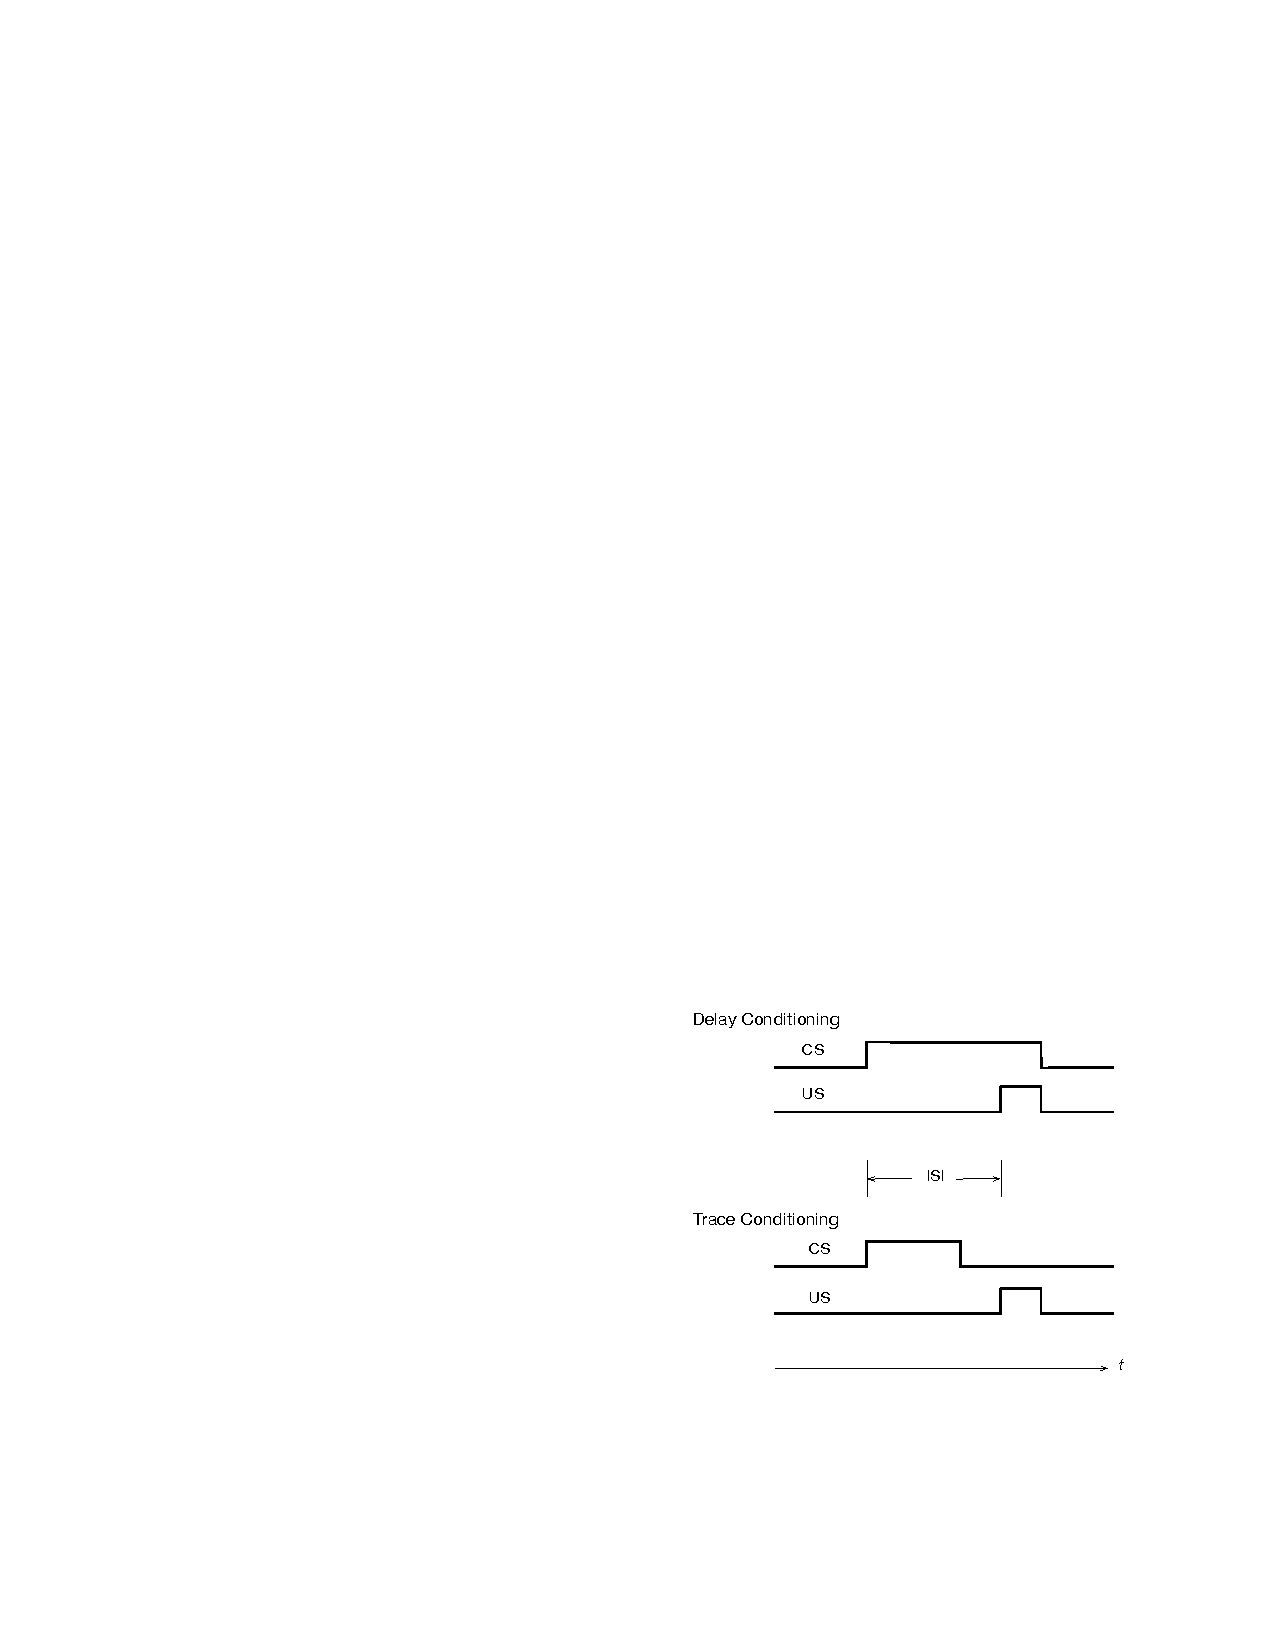
\includegraphics[width=0.5\linewidth]{chap11/fig_11_0}
	\caption{  \label{fig:11_0}}
\end{figure}


巴甫洛夫的狗对节拍器的声音流涎只是经典条件反射的一个例子,已经在许多动物的许多反应系统中进行了深入研究。
URs通常在某种程度上是准备性的,比如巴甫洛夫的狗流涎,或者在某种程度上是保护性的,比如对刺激眼睛的东西眨眼,或者看到捕食者时冻结。
在一系列试验中经历CS-US预测关系会使动物了解到CS预测美国,因此动物可以通过CR对CS做出反应,为动物做好准备或保护其免受预测的美国的影响。
一些CR类似于UR,但开始得更早,并且以增加其有效性的方式开始。
例如,在一项深入研究的实验中,音调CS可靠地预测了兔子眼睛的空气pu(美国),触发了UR,该UR由称为切口膜的保护性内眼睑闭合组成。
在一次或多次试验后,音调开始触发由膜闭合组成的CR,该膜闭合在空气pu之前开始并最终定时,以便在空气pu可能发生时发生峰值闭合。
这种CR是在预期空气pu和适当时间的情况下启动的,比简单地启动关闭作为对刺激我们的反应更好。通过学习刺激之间的预测关系来预测重要事件的能力是如此有益,它广泛存在于动物界。





\subsection{阻塞和高阶条件反射}

在实验中已经观察到经典条件反射的许多有趣性质。
除了CRs的预期性质之外,在经典调节模型的发展中,两个广泛观察到的特性得到了显着体现:阻塞和高阶调节。
当一个潜在的CS与之前用于调节动物产生CR的另一个CS一起出现时,当动物无法学习CR时,就会发生阻塞。
例如,在涉及兔子切口膜调节的阻断实验的第一阶段,兔子首先用音调CS和空气pu US调节,以产生在预期空气pu的情况下关闭其切口膜的CR。
实验的第二阶段包括额外的试验,其中第二个刺激(例如光)被添加到音调中以形成复合音调/光CS,然后是相同的空气pu US。
在实验的第三阶段,仅第二个刺激(即光)被呈现给兔子,以查看兔子是否已经学会了用CR对其作出反应。
结果表明,兔子对光的反应产生了很少或没有CR:对光的学习已经被先前对音调的学习所阻止。
2这样的阻止结果挑战了这样的观点,即调节只依赖于简单的时间连续性,即必要和足够的条件条件反射是美国经常在时间上紧跟CS。
在下一节中,我们将描述Rescorla{Wagner模型(Rescorla和Wagner,1972),该模型为阻塞提供了全面的解释。
	


当先前条件化的CS充当US来调节另一个最初中性的刺激时,就会发生高阶条件化。
如上所述,巴甫洛夫描述了一个实验,在这个实验中,他的助手首先调节一只狗,让它随着节拍器的声音流涎,节拍器可以预测食物的味道。
在这个调节阶段之后,进行了许多试验,其中将狗最初独立的黑色方块放置在狗的视线中,然后是节拍器的声音,而不是食物。
在仅仅十次试验中,这只狗只在看到黑色方块时才开始流涎,尽管事实上,看到它之后从来没有食物。
节拍器的声音本身就像一个US,将流涎的CR调节为黑色方块CS。
这是二阶条件反射。如果黑色方块被用作美国来建立另一个中性CS的唾液CRs,那么它将是三阶条件反射,等等。高阶条件反射很难证明,特别是在二阶以上,部分原因是高阶增强剂由于在高阶条件反射试验中没有被原美国反复遵循而失去了增强价值。
但是在正确的条件下,例如将一阶试验与高阶试验混合或通过提供一般的激励刺激,可以证明二阶以上的高阶条件反射。
正如我们在下面所描述的,经典条件反射的TD模型使用了自举思想,这是我们的方法的核心,以扩展Rescorla{Wagner模型对阻塞的描述,以包括CRs的预期性质和高阶条件反射。
	
	
高阶仪器调节也会发生。
在这种情况下,持续预测初级强化的刺激本身就变成了强化剂,如果通过进化将其奖励或惩罚的品质建立在动物体内,则强化是主要的。
预测刺激成为二级增强剂,或者更一般地说,是高阶或条件性增强剂|当预测的增强刺激本身是二级或甚至更高阶的增强剂时,后者是更好的术语。
条件性强化剂提供条件性强化:条件性奖励或条件性惩罚。
条件性强化就像初级强化一样,增加动物产生导致条件性奖励的行为的倾向,并减少动物产生导致条件性惩罚的行为的倾向。
(请参阅本章末尾的评论,解释我们的术语有时与心理学中使用的术语有何不同。)



条件性强化是一个关键现象,它解释了为什么我们为条件性强化货币工作,而条件性强化货币的价值完全来自于拥有它所预测的东西。
在第13.5节描述的演员{批评家方法(并在第15.7节和第15.8节的神经科学背景下进行了讨论)中,批评家使用TD方法来评估演员的政策,其价值估计为演员提供了条件性强化,从而使演员能够改进其政策。
这种更高阶的工具性条件作用的类似物有助于解决第1.7节中提到的信贷分配问题,因为当主要奖励信号延迟时,评论家会对演员进行瞬间强化。
我们将在下面的第14节中对此进行更多讨论。四。


\subsection{雷斯科拉-瓦格纳模型}

Rescorla和Wagner创建模型主要是为了解释阻塞。
\textit{雷斯科拉-瓦格纳模型}的核心思想是,动物只有在事件违反其预期时才能学习,换句话说,只有当动物感到惊讶时(尽管不一定意味着任何有意识的期望或情绪)。
我们首先使用Rescorla和Wagner的术语和符号来呈现模型,然后再转向我们用来描述TD模型的术语和符号。


以下是Rescorla和Wagner如何描述他们的模型。
该模型调整化合物CS的每个成分刺激的“关联强度”,这是一个数字,表示该成分预测US的强度或可靠性。
当在经典调节试验中呈现由多个成分刺激组成的化合物CS时,每个成分刺激的关联强度的变化方式取决于与整个刺激化合物相关的关联强度,称为“聚合关联强度”,而不仅仅取决于每个成分本身的关联强度。


Rescorla和Wagner考虑了一种化合物CS AX,由成分刺激a和X组成,其中动物可能已经经历了刺激a,而刺激X可能是动物新的。设VA,VX和VAX分别表示刺激A,X和化合物AX的结合强度。
假设在试验中,化合物CS AX后面跟着一个US,我们将其标记为刺激Y。
然后刺激成分的关联强度根据以下表达式变化:

\begin{equation}
	\Delta V_A = \alpha_A \beta_Y
		(R_Y - V_{AX})
\end{equation}


\begin{equation}
	\Delta V_X = 
		\alpha_X \beta_Y
		(R_Y - V_{AX})
\end{equation}

其中A Y和X Y是步长参数,取决于CS分量和US的恒等式,Y是US Y可以支持的结合强度的渐近水平。
(Rescorla和Wagner在这里使用R代替R,但我们使用R是为了避免与我们使用and混淆,因为我们通常认为这是奖励信号的大小,但需要注意的是,经典条件反射中的美国不一定是奖励或惩罚的。)该模型的一个关键假设是总联想强度VAX等于VA+VX。
由这些s改变的关联强度在下一次试验开始时成为关联强度。


为了完成,该模型需要一种响应生成机制,这是一种将V s值映射到CR的方法。
因为这种映射将取决于实验情况的细节,所以Rescorla和Wagner没有指定映射,而是简单地假设较大的V s会产生更强或更可能的CRs,并且负V s意味着不会有CRs。


Rescorla{Wagner模型以一种解释阻塞的方式解释了CRs的获取。
只要刺激化合物的总结合强度VAX低于美国Y可以支持的结合强度RY的渐近水平,预测误差RY􀀀VAX为正。
这意味着在连续的试验中,成分刺激的关联强度VA和VX增加,直到总关联强度VAX等于RY,此时关联强度停止变化(除非美国改变)。当将新组分添加到动物已经调理过的化合物CS中时,用增强化合物进一步调理会使添加的CS组分的缔合强度几乎没有增加,或者没有增加,因为误差已经减小到零或低值。
美国的发生几乎已经被完美地预测到了,因此新的CS组件几乎没有引入错误或惊喜。先前的学习阻碍了对新组件的学习。


为了从Rescorla和Wagner的模型过渡到经典条件反射的TD模型(我们称之为TD模型),我们根据本书中使用的概念重新构建了他们的模型。
具体来说,我们将用于学习的符号与线性函数近似(第9.4节)相匹配,并且我们认为调节过程是在试验中基于该试验中提出的化合物CS“学习预测美国的大小”的过程之一,其中美国Y的大小是如上所述的Rescorla{Wagner模型的Y。
我们还引入了状态。因为Rescorla{Wagner模型是一个试验级模型,这意味着它处理了从试验到试验的联想强度如何变化,而不考虑试验内部和试验之间发生的任何细节,我们不必考虑在试验期间状态如何变化,直到我们在下一节。
相反,在这里,我们简单地将状态视为根据试验中存在的组件CSs的集合来标记试验的一种方式。


因此,假设试验类型或状态s由特征x(s)=(x1(s)的实值向量描述;x2(s);:::;xd(s))>如果试验中存在化合物CS的第i个组分CSi,则xi(s)=1,否则为0。
然后,如果结合强度的d维向量为w,则试验类型s的总结合强度为

\begin{equation}\label{key}
	v(s, \textbf{w}) = 
		w^T x(s).
\end{equation}
这对应于强化学习中的价值估计,我们认为它是美国的预测。

现在暂时让t表示完整试验的次数,而不是它作为时间步长的通常含义(当我们将其扩展到下面的TD模型时,我们恢复到t的通常含义),并假设St是对应于试验t的状态。
调节试验t将关联强度向量wt更新为wt+1,如下所示:

\begin{equation}\label{key}
	w_{t+1} = w_t + \alpha \delta_t x(S_t),
\end{equation}

步长参数在哪里,因为这里我们描述的是Rescorla{Wagner模型| t是预测误差
	
\begin{equation}\label{key}
	\delta = R_t - v (S_t, w_t).
\end{equation}


Rt是试验t预测的目标,即美国的规模,或者用Rescorla和Wagner的话说,是美国在试验中可以支持的联合强度。
请注意,由于(14.2)中的因子x(St),因此只有试验中存在的CS组件的关联强度才能作为该试验的结果进行调整。
你可以将预测误差视为惊喜的衡量标准,将总联想强度视为动物的期望,当它与美国的目标幅度不匹配时,就会被违反。


从机器学习的角度来看,Rescorla{Wagner模型是一种纠错监督学习规则。它本质上与最小均方(LMS)或Widrow-Ho学习规则(Widrow and Ho,1960)相同,该规则将权重(这里是关联强度),使所有误差的平方平均值尽可能接近零。
它是一种“曲线”或回归算法,广泛用于工程和科学应用(见第9.4节)。3


Rescorla{Wagner模型在动物学习理论的历史上是非常重要的,因为它表明一个“机械”理论可以解释关于阻塞的主要事实,而不需要诉诸更复杂的认知理论,例如,动物明确认识到另一个刺激成分已被添加,然后向后扫描其短期记忆,以重新评估涉及美国的预测关系。
Rescorla{Wagner模型显示了传统的连续性调节理论,即刺激的时间连续性是学习的必要和充分条件,可以通过一种简单的方式来调整,以解释阻塞(Moore和Schmajuk,2002年)2008年)。
	
	
Rescorla{Wagner模型提供了经典条件反射的阻塞和其他一些特征的简单说明,但它不是经典条件反射的完整或完美模型。
不同的想法解释了各种其他观察到的影响,并且在理解经典条件反射的许多微妙之处方面仍在取得进展。
我们接下来描述的TD模型虽然也不是经典条件反射的完整或完美模型,但它扩展了Rescorla{Wagner模型,以解决刺激之间的试验内和试验间的时间关系如何影响学习以及如何产生更高阶的条件反射。
	

\subsection{时间差分}

TD模型是一个实时模型,而不是像Rescorla{Wagner模型这样的试验级模型。在我们上面的Rescorla和Wagner模型的公式中,一个单步t代表了一个完整的条件反射试验。
该模型不适用于关于试验期间发生的事情或试验之间可能发生的事情的细节。
在每个试验中,动物可能会经历各种刺激,这些刺激的发作发生在特定的时间,并且具有特定的持续时间。
这些时间关系强烈影响学习。Rescorla{Wagner模型也不包括高阶条件反射的机制,而对于TD模型,高阶条件反射是TD算法基础上的自举思想。
	
	
	
为了描述TD模型,我们从上面的Rescorla{Wagner模型的公式开始,但t现在标记了试验内或试验之间的时间步长,而不是完整的试验。将t和t+1之间的时间想象为一个小的时间间隔,例如0.01秒,并将试验视为一系列状态,每个时间步长都有一个关联,其中步骤t的状态现在表示刺激在t处如何表示的细节,而不仅仅是试验中CS成分的标签。
事实上,我们可以完全放弃试验的想法。
从动物的角度来看,试验只是其与世界相互作用的持续经验的一部分。
遵循我们通常的观点一个与环境相互作用的主体,想象动物正在经历一系列无尽的状态s,每个状态s都由特征向量x(s)表示。也就是说,将试验称为实验中刺激模式重复的时间片段仍然很方便。


状态特征不限于描述动物经历的外部刺激;它们可以描述外部刺激在动物大脑中产生的神经活动模式,这些模式可能与历史有关,这意味着它们可能是由外部刺激序列产生的持续模式。
当然,我们不确切知道这些神经活动模式是什么,但是像TD模型这样的实时模型允许人们探索学习关于外部刺激的内部表征的不同假设的后果。
由于这些原因,TD模型不适用于任何特定的状态表示。
此外,由于TD模型包括跨越刺激之间时间间隔的折扣和资格痕迹,因此该模型还可以探索折扣和资格痕迹如何与刺激表征相互作用,以预测经典调节实验的结果。


下面我们描述了TD模型中使用的一些状态表示及其含义,但目前我们对表示不可知,只假设每个状态s由特征向量x(s)=(x1(s)表示;x2(s);:::;xn(s))>。
然后(14.1)给出了对应于状态s的总结合强度,与Rescorla-Wgner模型相同,但TD模型不同地更新了结合强度向量w。
t现在标记了一个时间步长而不是一个完整的试验,TD模型根据此更新来管理学习:

\begin{equation}\label{key}
	w_{t+1} = w_t + \alpha \delta_t z_t,
\end{equation}

它将Rescorla{Wagner update(14.2)中的xt(St)替换为合格跟踪向量zt,而不是(14.3)的t,这里t是TD错误:
	
	
\begin{equation}\label{key}
	\delta_t = 
		R_{t+1} + \gamma v (S_{t+1}, w_t) - v(S_t, w_t),
\end{equation}


其中是折扣因子(介于0和1之间),Rt是时间t的预测目标, v(St+1;wt)和 v(St;wt)是t+1和t的总结合强度,如(14.1)所定义的。


资格跟踪向量zt的每个分量i根据特征向量x(St)的分量xi(St)递增或递减,否则会以以下公式确定的速率衰减:

\begin{equation}\label{key}
	z_{t+1} = \gamma \lambda z_t 
		+ x(S_t).
\end{equation}

这是通常的资格跟踪衰减参数。

请注意,如果=0,TD模型将简化为Rescorla{Wagner模型,但以下情况除外:t的含义在每种情况下都是不同的(Rescorla{Wagner模型的试用号和TD模型的时间步长),并且在TD模型中,预测目标R中有一个时间步长领先。
TD模型相当于具有线性函数近似的半梯度TD()算法的后视图(第12章),除了模型中的Rt不必像TD算法用于学习用于政策改进的值函数时那样是奖励信号。



